\chapter{本論文の重要箇所のまとめ}

系の上下両端のポテンシャルエネルギー差と運動エネルギー差の比を

\begin{align}
  \chi &\equiv \frac{k_{\text{B}}\Delta T}{mgL_{y}} = 1.265
\end{align}

として重力と熱流を設定し, 

\begin{figure}[H]
  \centering
  \caption{系の概略図}
  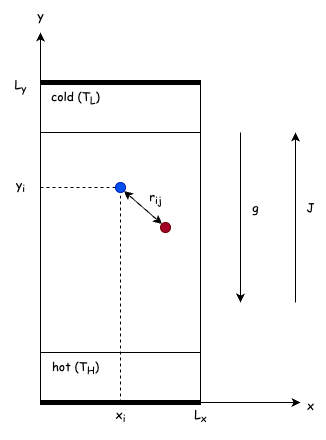
\includegraphics[scale=0.4]{image/system_pair.png}
\end{figure}

ハミルトニアンを

\begin{align}
  H(\Gamma; g)
  &= \sum_{i=1}^{N}
  \left[
    \frac{{\bm{p}_i}^2}{2m} 
    + \sum_{j > i}^{N}
      \tilde{\phi}_{\text{LJ}}^{\text{pair}}(r_{ij})
    + mgy_i
    + V^{\text{wall}} (y_i)
  \right] \ \tag*{\eqref{Hamiltonian}} 
\end{align}

とした(詳しくは\ref{chap:system}章を参照)系において, 

壁の親水性が高いほど, 流体系の重心位置は激しく変化し, 周期的なダイナミクスが現れるということがわかった. (詳しくは\ref{sec:CoM}節を参照.)

\begin{figure}[H]
  \begin{tabular}{cc}
    \begin{minipage}[t]{0.5\hsize}
      \centering
      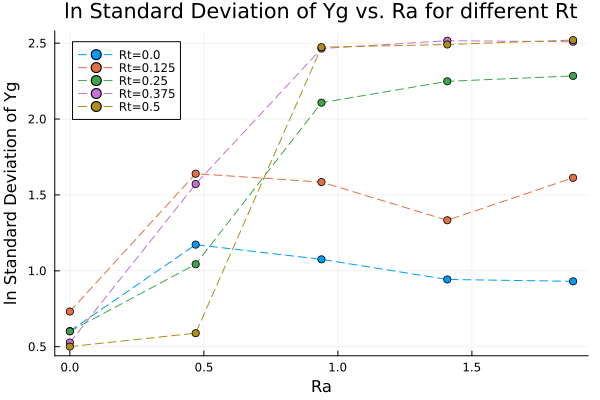
\includegraphics[width=\textwidth]{image/lnStdYg_Ra0.0to1.877538_Rt0.0to0.5_ti25000.png}
      \subcaption{横軸$\colon \text{R}_\text{a}$}
      \label{}
    \end{minipage}
    \begin{minipage}[t]{0.5\hsize}
      \centering
      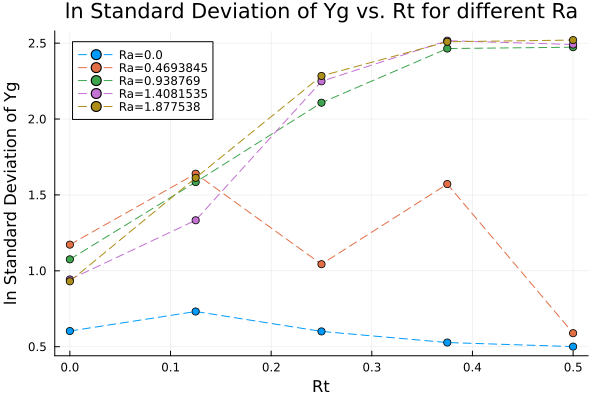
\includegraphics[width=\textwidth]{image/lnStdYg_Rt0.0to0.5_Ra0.0to1.877538_ti25000.png}
      \subcaption{横軸$\colon \text{R}_\text{t}$}
      \label{}
    \end{minipage}
  \end{tabular}
  \caption{縦軸:重心位置の標準偏差の対数プロット}
  \label{}
\end{figure}

また, 壁の濡れ性が大きく, ダイナミクスが現れるような流体系の重心位置と空間的なばらつきの相空間上での軌道は閉じることがわかった. (詳しくは\ref{sec:limitcycle}節を参照.)



\begin{figure}[H]
  \centering
  \begin{tabular}{ccc}
    \begin{minipage}[t]{0.3\hsize}
      \centering
      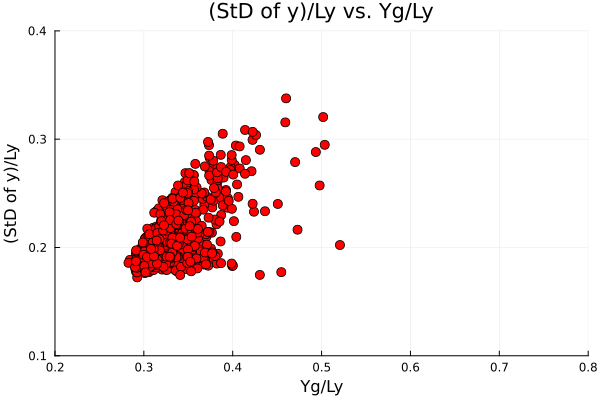
\includegraphics[width=\textwidth]{image/RaRtmap10_cycle/2023-12-28T12:38:51.436_map_10times_chi1.265_Ay50_rho0.4_T0.43_dT0.04_Rd0.0_Rt0.0_Ra1.877538_g0.0003999718779659611_run4.0e8.png}
      \subcaption{Ra1.877,Rt0.0}
      \label{}
    \end{minipage} &
    \begin{minipage}[t]{0.3\hsize}
      \centering
      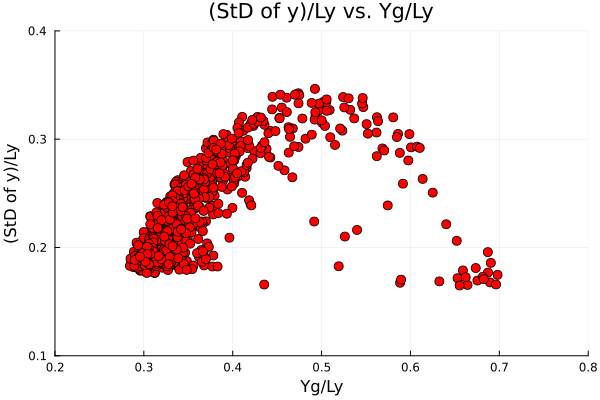
\includegraphics[width=\textwidth]{image/RaRtmap10_cycle/2023-12-28T12:38:51.827_map_10times_chi1.265_Ay50_rho0.4_T0.43_dT0.04_Rd0.0_Rt0.125_Ra1.877538_g0.0003999718779659611_run4.0e8.png}
      \subcaption{Ra1.877,Rt0.125}
      \label{}
    \end{minipage} &
    \begin{minipage}[t]{0.3\hsize}
      \centering
      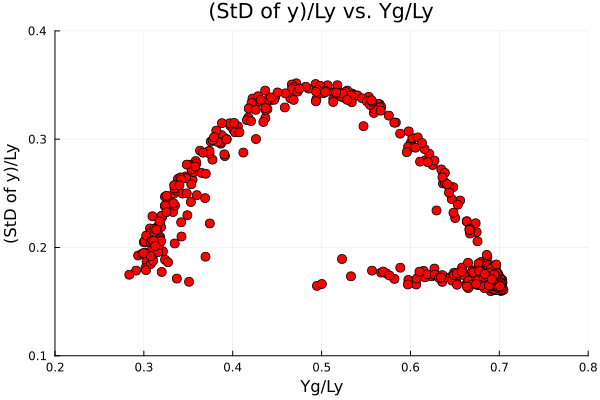
\includegraphics[width=\textwidth]{image/RaRtmap10_cycle/2023-12-28T12:38:52.986_map_10times_chi1.265_Ay50_rho0.4_T0.43_dT0.04_Rd0.0_Rt0.5_Ra1.877538_g0.0003999718779659611_run4.0e8.png}
      \subcaption{Ra1.877,Rt0.5}
      \label{}
    \end{minipage} 
  \end{tabular}
  \caption{リミットサイクル, Ra固定 $t_i = 4.0 \times 10^4 , t_f = 2.0 \times 10^6, t\sqrt{\epsilon/m{\sigma}^2} = 2000$ごとにプロット.}
\end{figure}

\begin{figure}[H]
  \centering
  \begin{tabular}{ccc}
    \begin{minipage}[t]{0.3\hsize}
      \centering
      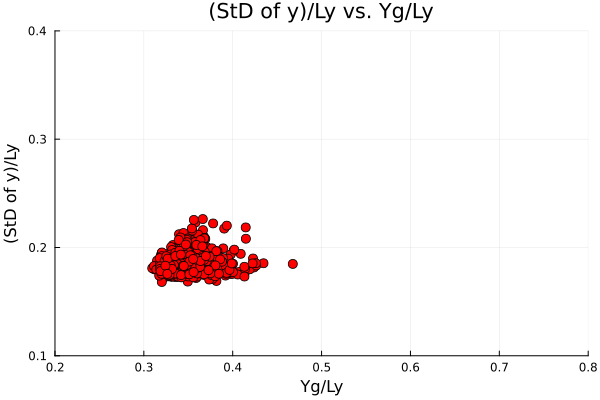
\includegraphics[width=\textwidth]{image/RaRtmap10_cycle/2023-12-28T12:38:52.686_map_10times_chi1.265_Ay50_rho0.4_T0.43_dT0.04_Rd0.0_Rt0.5_Ra0.0_g0.0003999718779659611_run4.0e8.png}
      \subcaption{Ra0.0,Rt0.5}
      \label{}
    \end{minipage} &
    \begin{minipage}[t]{0.3\hsize}
      \centering
      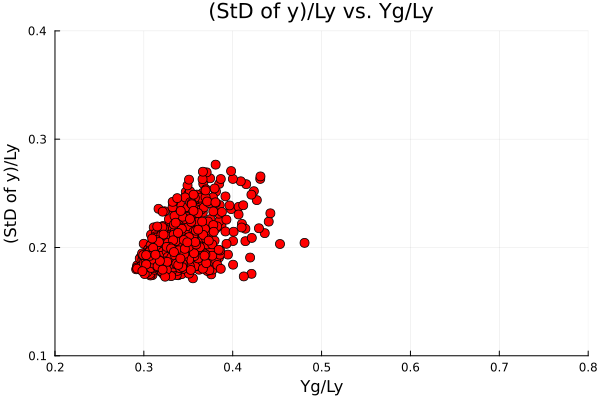
\includegraphics[width=\textwidth]{image/RaRtmap10_cycle/2023-12-28T12:38:52.752_map_10times_chi1.265_Ay50_rho0.4_T0.43_dT0.04_Rd0.0_Rt0.5_Ra0.4693845_g0.0003999718779659611_run4.0e8.png}
      \subcaption{Ra0.469,Rt0.5}
      \label{}
    \end{minipage} &
    \begin{minipage}[t]{0.3\hsize}
      \centering
      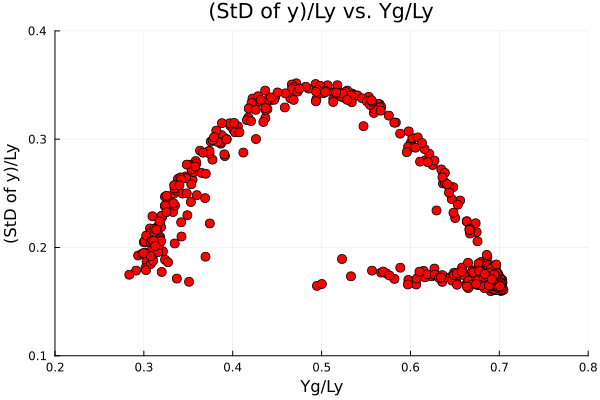
\includegraphics[width=\textwidth]{image/RaRtmap10_cycle/2023-12-28T12:38:52.986_map_10times_chi1.265_Ay50_rho0.4_T0.43_dT0.04_Rd0.0_Rt0.5_Ra1.877538_g0.0003999718779659611_run4.0e8.png}
      \subcaption{Ra1.877,Rt0.5}
      \label{}
    \end{minipage} 
  \end{tabular}
  \caption{リミットサイクル, Rt固定, $t_i = 4.0 \times 10^4 , t_f = 2.0 \times 10^6, t\sqrt{\epsilon/m{\sigma}^2} = 2000$ごとにプロット.}
\end{figure}